% partes/parte2/cap08.tex
\chapter{Figuras participantes en la decisión digital}
\label{cap:08}

\begin{cajaFicha}
\begin{description}
  \item[Unidad temática] II — Proceso de toma de decisión de compra digital.
  \item[Temas del programa] 2.3 Figuras participantes en la toma de decisiones digitales: 2.3.1 Consumidor / Usuario / \textit{Buyer persona} / Prosumidor; 2.3.2 Influenciador / \textit{Influencer}; 2.3.3 Decisor; 2.3.4 Comprador; 2.3.5 Evaluador.
  \item[Horas] Teoría 2.0 · Práctica 3.0 · Aprendizaje autónomo 1.0 (asignación tentativa; ver Anexo B del prompt de proyecto, anomalía 4).
  \item[Competencia de la unidad] Examina el proceso de toma de decisiones de compra del consumidor digital a partir de su recorrido y figuras participantes.
  \item[Resultados de aprendizaje observables] Al concluir el capítulo, el estudiante:
  \begin{enumerate}
    \item distingue siete figuras (consumidor, usuario, prosumidor, influenciador, decisor, comprador, evaluador) y reconoce que una persona puede reunir varias;
    \item explica el origen y los límites del \textit{buyer persona};
    \item calcula tres medidas de centralidad en una red y explica por qué tener muchos seguidores no equivale a influir;
    \item simula una cascada de adopción por umbral y compara tres formas de elegir a las personas semilla.
  \end{enumerate}
  \item[Prerrequisitos] Cap. 1--7.
\end{description}
\end{cajaFicha}

\section{Caso de apertura}

\begin{casoFicticio}
Valeria cumple quince años y quiere una consola de videojuegos. Pasa dos
semanas viendo videos de una creadora de contenido a la que sigue desde hace
años. Su padre, Rodolfo, es quien elige el presupuesto y revisa tres
comparativos en línea para decidir el modelo. Su tía Ángeles lo ordena en una
tienda y lo paga con su tarjeta, porque tiene un descuento. Valeria,
además, publica reseñas de los juegos que prueba; la creadora ya citó una.

Una sola compra. Cinco personas con cinco papeles distintos.
\end{casoFicticio}

La mercadotecnia suele hablar de \enquote{el consumidor} como si fuera una
sola persona que ve, decide, paga y usa. Casi nunca ocurre así. El caso de
Valeria separa lo que el lenguaje cotidiano mezcla: quien usa, quien influye,
quien decide, quien paga y quien compara. Cada papel deja un rastro de datos
distinto y exige una estrategia distinta. Un anuncio dirigido a Valeria no
convence a Rodolfo, y una reseña de Valeria puede pesar más que el anuncio.

\section{Desarrollo teórico}

La figura~\ref{fig:cap08-roles} resume las siete figuras que el programa
distingue. Ninguna describe a una \emph{persona}; describen \emph{papeles}. Una
misma persona puede reunir varios, y un mismo papel puede repartirse entre
varias personas. En compra organizacional, la literatura clásica llama
\enquote{centro de compra} (\textit{buying center}) al conjunto de personas
que comparten esas funciones \parencite{webster1972}; el consumo individual y
familiar hereda la idea.

\begin{figure}[!htb]
  \centering
  \resizebox{0.95\textwidth}{!}{% figuras/tikz/cap08-figuras-participantes.tex
% Figuras que participan en una decisión de compra digital. Una misma persona
% puede jugar varios roles; un rol puede repartirse entre varias personas.
\begin{tikzpicture}[
    rol/.style={rectangle, rounded corners, draw=guindaIPN, thick, fill=guindaIPNClara,
                minimum width=3.0cm, minimum height=1.15cm, align=center, font=\scriptsize},
    rolD/.style={rectangle, rounded corners, draw=bronceIPN, thick, fill=bronceIPNClaro,
                 minimum width=3.0cm, minimum height=1.15cm, align=center, font=\scriptsize},
    centro/.style={ellipse, draw=guindaIPN, very thick, fill=white, minimum width=3.2cm, minimum height=1.6cm, align=center, font=\small\bfseries},
    flecha/.style={-{Stealth[length=2.3mm]}, thick, draw=doradoIPN},
    nota/.style={font=\tiny, text=grisIPN, align=center}
  ]
  \node[centro] (c) at (0,0) {Decisión\\ de compra};
  \node[rol]  (u)  at (-5.2,2.6)  {\textbf{Usuario}\\ usa el producto};
  \node[rol]  (co) at (-5.2,0)    {\textbf{Consumidor}\\ consume y se beneficia};
  \node[rolD] (pr) at (-5.2,-2.6) {\textbf{Prosumidor}\\ también produce contenido};
  \node[rol]  (i)  at (0,3.6)     {\textbf{Influenciador}\\ orienta a otros};
  \node[rol]  (e)  at (0,-3.6)    {\textbf{Evaluador}\\ compara y pondera (persona o IA)};
  \node[rol]  (d)  at (5.2,2.6)   {\textbf{Decisor}\\ elige qué y cuándo};
  \node[rol]  (cm) at (5.2,-2.6)  {\textbf{Comprador}\\ paga y ejecuta la compra};
  \foreach \n in {u,co,pr,i,e,d,cm} { \draw[flecha] (\n) -- (c); }
  \node[rolD, dashed] (bp) at (5.2,0) {\textbf{\textit{Buyer persona}}\\ arquetipo de la organización};
  \draw[-{Stealth[length=2.3mm]}, thick, dashed, draw=bronceIPN] (bp) -- (c);
  \node[nota] at (0,-5.0) {Una misma persona puede ser usuaria, decisora y compradora; en otras compras estos roles se reparten.};
\end{tikzpicture}
}
  \caption{Figuras participantes en la decisión de compra digital. Fuente:
  elaboración propia; la noción de papeles repartidos procede del centro de
  compra de \textcite{webster1972}.}
  \label{fig:cap08-roles}
\end{figure}

\subsection{Consumidor, usuario, \textit{buyer persona} y prosumidor}
\progtag{2.3.1}
\label{sec:cap08-persona}

\textbf{Consumidor y usuario.} El \emph{consumidor} es quien se beneficia del
producto o servicio; el \emph{usuario}, quien lo utiliza. Coinciden en un
cuaderno y divergen en un servicio por suscripción corporativa, donde quien usa
no es quien decide ni quien paga. La distinción importa porque los datos de
uso describen al usuario, y los de compra, al comprador.

\textbf{\textit{Buyer persona}.} \textcite{cooper1999inmates} propuso la
\enquote{persona} como arquetipo de diseño de software: un personaje
construido para orientar decisiones de diseño. El término \enquote{\textit{buyer
persona}} es una adaptación posterior a la mercadotecnia; la literatura
consultada para este libro la sitúa entre 2000 y 2001, con firmas como
Pragmatic Marketing y Forrester. Cooper no lo usó con ese nombre. Conviene
separar tres cosas que la práctica mezcla. La persona es un
\emph{arquetipo ficticio}. El segmento es un \emph{grupo real} de clientes. El
cliente individual es una \emph{persona concreta}. Confundir la primera con
la tercera es el error más frecuente: una persona con nombre, foto y
aficiones se parece mucho a alguien, y por eso convence más de lo que
demuestra.

\textbf{Prosumidor.} \textcite{toffler1980thirdwave} acuñó \textit{prosumer}
(productor y consumidor) para describir la disolución de la frontera entre
producir y consumir. El fenómeno no es nuevo: la economía de autoconsumo
preindustrial lo practicaba. Lo que la tecnología digital reactivó fue su
escala. Hoy se manifiesta en reseñas, contenido generado por usuarios,
creación en redes y codiseño de producto. En el caso de apertura, Valeria es
prosumidora: consume los juegos y produce reseñas que otros leen.

\begin{cajaFrontera}
\textbf{Personas sintéticas con modelos de lenguaje.} Una propuesta reciente
sustituye al \textit{buyer persona} dibujado a mano por \enquote{muestras de
silicio}: un modelo de lenguaje al que se le pide responder como lo haría una
persona con cierto perfil demográfico. \textcite{argyle2023} mostraron que, en
ciertos temas de opinión política, un modelo condicionado con perfiles
demográficos reproduce patrones de respuesta de subgrupos reales; llamaron a
esa propiedad \enquote{fidelidad algorítmica}.

El resultado no se generaliza sin cuidado. \textcite{bisbee2024} pidieron a un
modelo que generara valoraciones de grupos sociopolíticos y las compararon
con una encuesta nacional estadounidense: los promedios se parecían, pero
las respuestas sintéticas variaban menos y los coeficientes de regresión
diferían de los reales con frecuencia. Además, el resultado cambiaba con
pequeñas variaciones del texto de la instrucción y con el paso de los meses.
Los autores concluyen que esos datos son poco confiables para la inferencia
estadística. Para la mercadotecnia, el uso razonable hoy es exploratorio:
generar hipótesis para contrastar con personas reales, no sustituirlas. Es
el mismo criterio que se aplica al \textit{buyer persona} tradicional.
\end{cajaFrontera}

\subsection{Influenciador}
\progtag{2.3.2}
\label{sec:cap08-influ}

Un \emph{influenciador} es quien orienta las decisiones de otros por la
credibilidad, el atractivo o la cercanía que su audiencia le atribuye. La
figura tiene un antecedente en el líder de opinión de la comunicación
interpersonal y en el modelo del flujo en dos pasos
\parencite{lazarsfeld1944peopleschoice,katzlazarsfeld1955}: la
información de los medios llega a muchas personas a través de otras que la
filtran. Lo que cambia hoy es la escala y la distancia con la audiencia. La
etiqueta cubre figuras muy distintas, y el tamaño de la audiencia es la
forma más usada de clasificarlas: \emph{nano} (de mil a diez mil
seguidores), \emph{micro}, \emph{macro} y \emph{mega}. Los dos metaanálisis
más sólidos disponibles agrupan cientos de tamaños de efecto: 1\,531 de 251
estudios \parencite{leung2022influencer} y 571 de 71 artículos
\parencite{barari2025influencer}. Convergen en que el efecto opera
sobre todo por la credibilidad y el atractivo percibidos, y en que las
características de los seguidores predicen mejor la actitud, mientras que las del
contenido predicen mejor la intención de compra.

En México, la Procuraduría Federal del Consumidor publicó en 2023 la Guía de
Publicidad para Influencers \parencite{profeco2023influencers}. Recomienda
identificar el contenido pagado de forma visible durante toda su duración y
sugiere etiquetas estandarizadas (\textit{\#Publicidad}, \textit{\#Patrocinio},
entre otras). Es una \emph{guía de recomendaciones} con fundamento en la Ley
Federal de Protección al Consumidor, no una ley específica con régimen
sancionador propio; presentarla como ley sobrerrepresenta la regulación
vigente.

\begin{cajaFrontera}
\textbf{Comercio social, \textit{live commerce} y economía de creadores.} El
comercio social permite comprar sin salir de la red en que se descubre el
producto; el \textit{live commerce} vende en transmisión en vivo con
interacción en tiempo real. Fuentes secundarias de industria reportan que el
comercio social global habría pasado de unos 81 mil millones de dólares
en 2018 a unos 688 mil millones en 2024, y que las tasas de interacción
bajan con el tamaño de la audiencia (alrededor de 2.7\,\% en
nanoinfluenciadores frente a menos de 1\,\% en macroinfluenciadores). Estas
cifras fueron revisadas y confirmadas por el autor, pero no se localizó el
informe primario que las origina; deben leerse como órdenes de magnitud y no
como mediciones precisas.

Los metaanálisis arbitrados citados arriba ubican el efecto en mecanismos
de credibilidad y atractivo percibidos; esos mecanismos, y no el número de
seguidores, son lo que conviene evaluar antes de contratar. La consecuencia
para el recorrido (Cap.~7) es doble. Por un lado, un influenciador
pequeño puede ser un \emph{punto de contacto} de confianza, hipótesis que
cada marca debe contrastar con sus propios datos. Por otro, el creador
profesionalizado es, en sentido estricto, un
prosumidor que vive de su audiencia y tiene incentivos comerciales que la
transparencia publicitaria obliga a declarar.
\end{cajaFrontera}

\subsection{Decisor, comprador y evaluador}
\progtag{2.3.3}\progtag{2.3.4}\progtag{2.3.5}

El \emph{decisor} es quien determina si se compra, qué y cuándo. El
\emph{comprador} es quien ejecuta la transacción y paga. El \emph{evaluador}
es quien compara las alternativas y pondera sus atributos. En el caso de
apertura, el padre decide el presupuesto, la tía compra y los comparativos
evalúan. En la mayoría de las compras individuales los tres papeles
coinciden en una persona, y por eso se omiten; reaparecen en compras de
hogar, regalos, productos para menores y todo el comercio entre empresas.

La figura del \emph{evaluador} es la que más cambia en digital. Antes era
casi siempre una persona (un vendedor, un amigo). Hoy puede ser un tercero
humano (reseñista, comparador de precios) o un asistente de inteligencia
artificial que resume y pondera opciones antes de que alguien decida
(Cap.~4). Cuando el evaluador es un sistema, la pregunta del
Cap.~6 vuelve con otra forma: ¿con qué regla de decisión pondera, y quién la
configuró? El cuadro~\ref{tab:cap08-roles} resume qué pregunta responde cada
figura y qué dato deja.

\begin{table}[!htb]
\centering
\begin{tabular}{@{}p{2.3cm}p{3.7cm}p{3.5cm}p{2.9cm}@{}}
\toprule
Figura & Pregunta que responde & Ejemplo digital & Dato que deja \\
\midrule
Usuario & ¿Quién usa el producto? & Perfil de uso de una aplicación & Eventos de uso \\
Consumidor & ¿Quién se beneficia? & Estudiante que consume un servicio & Satisfacción, recompra \\
Prosumidor & ¿Quién también produce? & Reseña, \textit{unboxing}, contenido propio & Contenido generado \\
Influenciador & ¿Quién orienta a otros? & Creador con audiencia & Alcance, interacción \\
Decisor & ¿Quién elige? & Quien aprueba el presupuesto & A menudo, ninguno visible \\
Comprador & ¿Quién paga? & Titular de la tarjeta & Transacción \\
Evaluador & ¿Quién compara? & Comparador, reseñista o asistente de IA & Búsquedas, comparaciones \\
\bottomrule
\end{tabular}
\caption{Siete figuras y el dato que cada una deja. Fuente: elaboración propia.}
\label{tab:cap08-roles}
\end{table}

\section{Evidencia de México y del mundo}

El grupo de edad con mayor uso de internet en México es el de 15 a 24 años,
con 97.6\,\% en 2025 \parencite{inegi2026endutih}. Es el grupo que concentra a
quienes consumen y producen contenido y que, con frecuencia, \emph{influye}
en las compras de su hogar sin ser quien paga. En el caso de Valeria, el
dato no le dice a la marca a quién dirigirse; le dice dónde buscar a quien
orienta la decisión.

La evidencia internacional más sólida es la de los metaanálisis ya citados
\parencite{leung2022influencer,barari2025influencer}. Su aporte más útil
para el estudiante no es una cifra, sino una advertencia: el efecto del
influenciador es heterogéneo y depende de mecanismos (credibilidad,
atractivo, identidad social de los seguidores). Elegir a un influenciador
por su número de seguidores ignora esos mecanismos, y esa es la
conclusión del laboratorio de este capítulo.

\section{Laboratorio MATLAB: ¿quién influye en una red social?}
\label{sec:cap08-lab}

\begin{cajaLaboratorio}
\textbf{Objetivo.} Generar una red social sintética con grupos, medir la
centralidad de cada persona, y simular una cascada de adopción para
comparar tres formas de elegir a las personas semilla: las más centrales,
las menos centrales y al azar.

\textbf{Concepto detrás del código.} Una red es un conjunto de personas
(nodos) y relaciones (aristas). El \emph{grado} cuenta las conexiones de cada
persona; es la medida más cercana a \enquote{seguidores}. La
\emph{intermediación} de una persona suma, sobre todos los pares de otras
personas, la fracción de los caminos más cortos entre ellas que pasa por
ella \parencite{brandes2001}; mide quién es \emph{puente}. La
\emph{cercanía} es el inverso de la distancia media a todos los demás.

La cascada sigue un modelo de umbral \parencite{granovetter1978}: cada
persona adopta cuando al menos una fracción $\theta$ de sus contactos ya
adoptó. Si $a_i(t)$ indica que la persona $i$ adoptó en la ronda $t$ y $N(i)$
es su conjunto de contactos,
\[
  a_i(t+1)=1 \iff a_i(t)=1 \;\text{ o }\; \frac{1}{|N(i)|}\sum_{j\in N(i)} a_j(t)\ \ge\ \theta .
\]
El proceso se repite hasta que nadie más adopta. Las semillas son las
personas que adoptan en la ronda 0.

\textbf{Script.} \texttt{matlab/cap08/cap08\_red\_influencia.m}. Es el
\textbf{mismo script, sin modificar}, que se usa en la práctica
\enquote{Recorrido del consumidor digital}. La red es \textbf{sintética}
(\texttt{rng(42)}): tiene grupos densos unidos por unas pocas conexiones y no
representa ninguna plataforma ni persona reales.

\begin{lstlisting}[style=MATLABStyle, caption={Bloque de parámetros editable (\texttt{cap08\_red\_influencia.m}) — es lo único que cambia entre corridas.}]
nNodos = 60;           % numero de personas en la red (30 a 100)
nComunidades = 3;      % grupos en que se reparte la gente (2 a 5)
pDentro = 0.20;        % prob. de que dos personas del mismo grupo se conozcan
pEntre = 0.01;         % prob. de que dos personas de grupos distintos se conozcan
nSemillas = 3;         % personas a las que se muestra el producto (1 a 10)
umbral = 0.25;         % fraccion de contactos que deben haber adoptado
criterio = 1;          % 1 grado, 2 intermediacion, 3 cercania
\end{lstlisting}

\textbf{Salida esperada.} Dos figuras: la red con las semillas y el
resultado de la cascada (figura~\ref{fig:cap08-red}) y la comparación entre
conexiones e intermediación y entre criterios de semilla
(figura~\ref{fig:cap08-seguidores}).

\begin{center}
  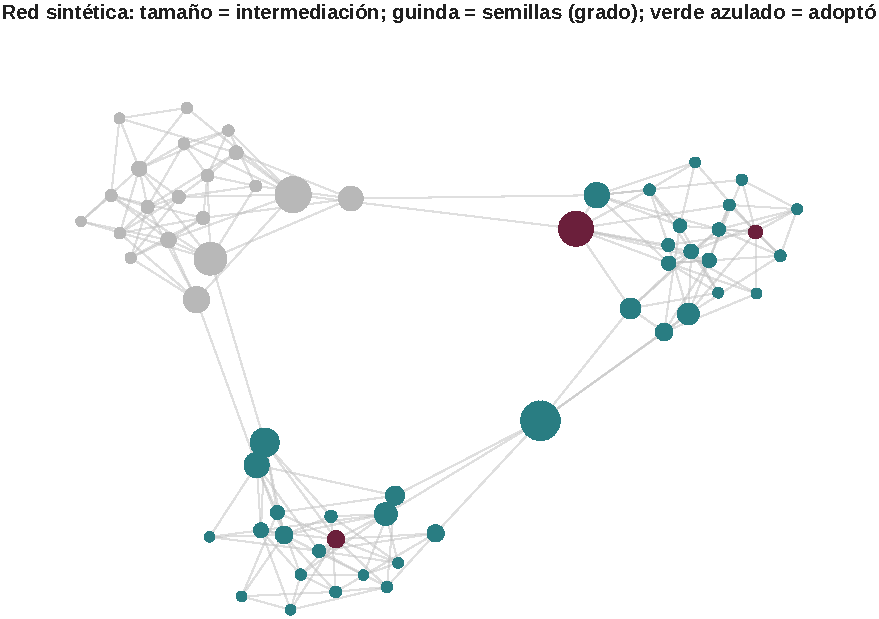
\includegraphics[width=0.92\textwidth]{figuras/matlab/cap08_red_influencia.pdf}
  \captionof{figure}{Red sintética de 60 personas en tres grupos. Tamaño:
  intermediación; guinda: semillas elegidas por grado; verde azulado:
  adoptó. Fuente: elaboración propia con datos sintéticos, \texttt{rng(42)}.}
  \label{fig:cap08-red}
\end{center}

\begin{center}
  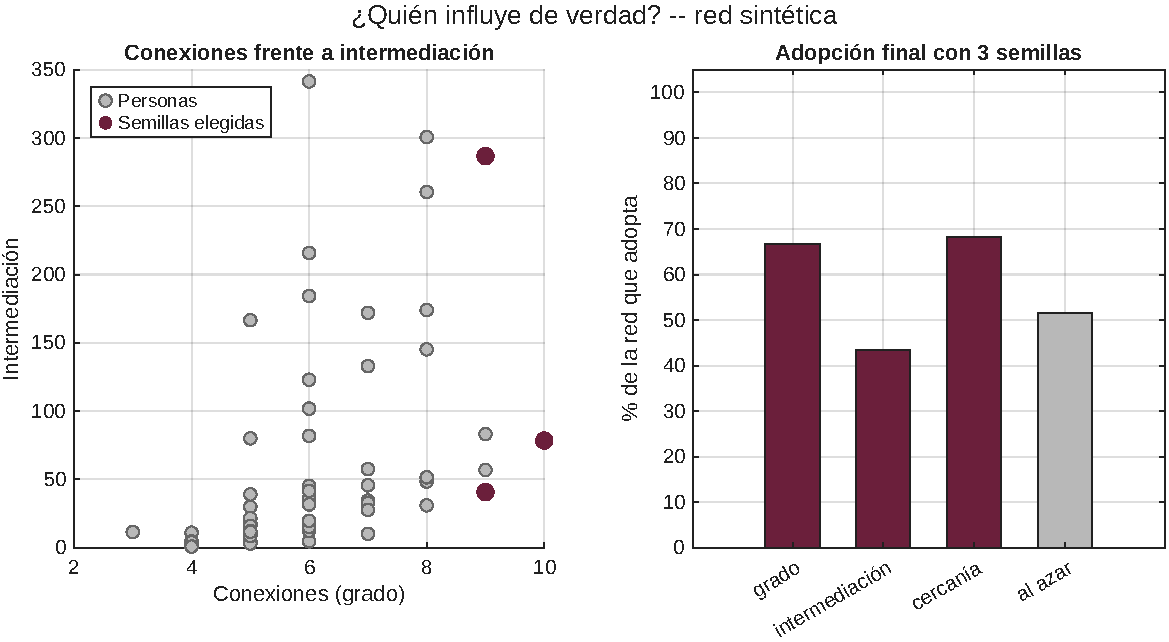
\includegraphics[width=0.92\textwidth]{figuras/matlab/cap08_seguidores_vs_influencia.pdf}
  \captionof{figure}{Conexiones frente a intermediación y adopción final
  según el criterio de semillas. Fuente: elaboración propia con datos
  sintéticos, \texttt{rng(42)}.}
  \label{fig:cap08-seguidores}
\end{center}

\textbf{Interpretación de negocio.} Con los valores por defecto, la lista de
las cinco personas con más conexiones y la de las cinco con más intermediación
coinciden en una sola. Tener muchos seguidores no es lo mismo que ser puente.
La figura~\ref{fig:cap08-puente} ilustra la diferencia: la persona \emph{H}
tiene más conexiones, pero todo camino entre los dos grupos pasa por la
persona \emph{P}.

\begin{center}
  \resizebox{0.8\textwidth}{!}{% figuras/tikz/cap08-puente-comunidades.tex
% Seguidores no es influencia: el nodo con más conexiones no es el único camino
% entre grupos. El puente tiene pocas conexiones y mucha intermediación.
\begin{tikzpicture}[
    n/.style={circle, draw=grisIPN, fill=guindaIPNClara, minimum size=0.55cm, inner sep=0pt},
    hub/.style={circle, draw=guindaIPN, very thick, fill=guindaIPN!35, minimum size=0.95cm, inner sep=0pt, font=\scriptsize\bfseries},
    puente/.style={circle, draw=bronceIPN, very thick, fill=bronceIPNClaro, minimum size=0.75cm, inner sep=0pt, font=\scriptsize\bfseries},
    arista/.style={draw=grisIPN!70, thick}
  ]
  % grupo A
  \node[hub] (a0) at (-3.4,0.2) {H};
  \foreach \i/\x/\y in {1/-4.8/1.2,2/-4.9/-0.7,3/-3.2/1.6,4/-2.6/-1.0,5/-4.0/-1.6,6/-5.4/0.3} {
    \node[n] (a\i) at (\x,\y) {};
    \draw[arista] (a0) -- (a\i);
  }
  \draw[arista] (a1) -- (a6) (a2) -- (a6) (a3) -- (a1);
  % grupo B
  \node[n] (b0) at (3.4,0.2) {};
  \foreach \i/\x/\y in {1/4.8/1.2,2/4.9/-0.7,3/3.2/1.6,4/2.6/-1.0,5/4.0/-1.6} {
    \node[n] (b\i) at (\x,\y) {};
    \draw[arista] (b0) -- (b\i);
  }
  \draw[arista] (b1) -- (b3) (b2) -- (b5) (b4) -- (b5);
  % puente
  \node[puente] (p) at (0,0.2) {P};
  \draw[arista] (a4) -- (p) (a3) -- (p) (p) -- (b4) (p) -- (b3);
  \node[font=\tiny, text=guindaIPN, align=center, text width=3.3cm] at (-4.1,-2.6) {\textbf{H}: más conexiones\\ (grado alto)};
  \node[font=\tiny, text=bronceIPN, align=center, text width=3.3cm] at (0,-2.6) {\textbf{P}: pocas conexiones;\\ todo camino entre grupos pasa por ella\\ (intermediación alta)};
  \node[font=\tiny, text=grisIPN, align=center, text width=3.3cm] at (4.1,-2.6) {Otro grupo};
\end{tikzpicture}
}
  \captionof{figure}{Grado frente a intermediación. Fuente: elaboración propia.}
  \label{fig:cap08-puente}
\end{center}

El resultado de la cascada es menos intuitivo. Con semillas elegidas por
grado se adopta 66.7\,\% de la red; con semillas elegidas por
intermediación, 43.3\,\%, menos que el 51.5\,\% promedio de elegirlas al azar. La
explicación probable es que el puente conecta grupos, pero un modelo de umbral exige que varios contactos
adopten antes de que alguien lo haga, y una persona-puente tiene pocos
contactos dentro de cada grupo. La medida adecuada depende del
\emph{mecanismo de contagio}. Para difundir información sencilla (compartir
un enlace), los puentes ayudan; para decisiones que exigen validación social
(comprar un producto), pesan más los contactos densos. Es una red sintética: lo
que se aprende es el método de comparación, no un orden universal de medidas.

\textbf{Ejercicio propuesto (usen exactamente este script, solo cambien el
bloque de parámetros).} Corran el script tres veces y completen un cuadro con
el número de conexiones, cuántas personas coinciden en los dos rankings, y
la adopción final con semillas por grado, por intermediación y al azar:
\begin{enumerate}
  \item \textbf{Caso A — valores por defecto:} los siete parámetros tal como
  están.
  \item \textbf{Caso B — más puentes:} cambien \texttt{pEntre} de 0.01 a
  0.06, sin tocar nada más.
  \item \textbf{Caso C — grupos más densos:} regresen \texttt{pEntre} a 0.01
  y cambien \texttt{pDentro} de 0.20 a 0.35.
\end{enumerate}
Con el cuadro completo, respondan por escrito: en el Caso B, ¿qué ocurre con
la adopción con semillas centrales y con la de semillas al azar, y qué papel
juegan los puentes? En el Caso C, ¿por qué una red más densa dificulta la
cascada con el mismo umbral? A partir de sus tres corridas, expliquen por qué
no basta con contratar a quien tiene más seguidores.

\textbf{Extensión opcional.} Cambien \texttt{criterio} a 2 y 3 en el Caso A,
y compárenlos con el criterio 1. ¿Cuál mide mejor la \enquote{influencia} en
una cascada por umbral? ¿Y en una de información simple?

\textbf{Sin MATLAB.}
\texttt{matlab/cap08/cap08\_red\_influencia\_interactivo.html} tiene los mismos
parámetros, los casos A, B y C, el dibujo de la red y los 100 sorteos al
azar.

\textbf{Con datos propios (extensión opcional).}
\texttt{cap08\_red\_datos\_propios.html}
analiza una red propia (hoja «Conexiones» con dos columnas, una conexión por fila, y hoja «Personas» opcional con el grupo de cada una) con las mismas medidas y la misma cascada: grado, intermediación, cercanía, semillas centrales, periféricas y 100 sorteos al azar. Identifiquen a las personas con seudónimos; los datos no salen del navegador.
\end{cajaLaboratorio}

\begin{cajaEtica}
Un grafo de relaciones revela más que los datos de cada persona. Quien
aparece como contacto de otra no consintió ser analizado: la red expone a
terceros. Elegir \enquote{semillas} por centralidad significa estudiar y
tratar de forma distinta a quienes ocupan posiciones clave, sin que
lo sepan. Y contratar a un influenciador exige transparencia: la guía de
PROFECO \parencite{profeco2023influencers} pide identificar el contenido
pagado, porque la credibilidad que se compra es la que su audiencia cree
gratuita. Antes de mapear una red real conviene preguntar quién queda
expuesto, con qué base legal (Cap.~3) y para qué decisión.
\end{cajaEtica}

\section{Estudio de caso}
\label{sec:cap08-caso}

\begin{casoFicticio}
Una marca mexicana de cosméticos tiene presupuesto para una campaña de
lanzamiento. Su agencia propone dos opciones: pagar a una macroinfluenciadora
con dos millones de seguidores, o repartir el mismo presupuesto entre doce
microinfluenciadoras de entre veinte y cincuenta mil seguidores cada una,
pertenecientes a seis comunidades de aficionados distintas. La agencia
sugiere elegir la primera \enquote{por alcance}.

Un analista de la marca obtiene datos de grupos de interés públicos y
reconstruye una red simplificada: las microinfluenciadoras conectan
comunidades que apenas se tocan entre sí; la macroinfluenciadora pertenece
a una sola comunidad grande.

\textbf{Preguntas guía.}
\begin{enumerate}
  \item ¿Qué medida de centralidad ayudaría a decidir entre ambas opciones y
  por qué?
  \item Si el producto exige validación social (probar y comparar con
  conocidas) antes de comprar, ¿qué le dice el laboratorio sobre elegir
  semillas por grado o por intermediación?
  \item ¿Qué datos debería pedir la marca a cada influenciadora y qué
  obligaciones de transparencia publicitaria aplican?
  \item ¿Qué riesgos éticos tiene que el analista reconstruya la red a partir
  de grupos públicos?
\end{enumerate}
\end{casoFicticio}

\section{Actividades y evidencias del portafolio}

Estas actividades hacen crecer el entregable único de la práctica
\enquote{Recorrido del consumidor digital}.

\begin{description}
  \item[Infografía colaborativa] Representar, para el caso real del equipo, las
  figuras participantes (usuario, consumidor, prosumidor, influenciador,
  decisor, comprador y evaluador), indicando qué persona o canal ocupa cada
  una y qué dato deja (cuadro~\ref{tab:cap08-roles}).
  \item[Reporte de investigación] Describir al \textit{buyer persona} que la
  organización del caso usaría y declarar tres limitaciones del arquetipo
  frente a clientes reales (sección~\ref{sec:cap08-persona}).
  \item[Solución de casos] Resolver por escrito el estudio de caso de la marca
  de cosméticos (sección~\ref{sec:cap08-caso}).
  \item[Reporte de práctica] Incluir el cuadro de los tres casos del
  laboratorio y las respuestas de comparación en el entregable único.
\end{description}

\section{Ruta de aprendizaje autónomo}

Una hora de aprendizaje autónomo. Tarea concreta:
\begin{enumerate}
  \item Ejecutar \texttt{cap08\_red\_influencia\_interactivo.html}, completar el
  cuadro de los casos A, B y C y comparar los tres criterios de semilla con
  el histograma de los 100 sorteos al azar. Anotar en dos líneas por qué una
  sola muestra aleatoria no sirve como referencia.
  \item (Opcional) Con \texttt{cap08\_red\_datos\_propios.html} (opcional), cargar el \textbf{Ejemplo 2} (club de aficionados) y comparar qué criterio de semillas rinde más.
\end{enumerate}

\section{Síntesis}

Una decisión de compra rara vez la toma una sola persona. Siete figuras
participan: usuario, consumidor, prosumidor, influenciador, decisor, comprador
y evaluador. Cada una deja un dato distinto y responde una pregunta distinta.
El \textit{buyer persona} es un arquetipo de diseño adaptado a la
mercadotecnia, no un cliente real, y los intentos de sustituirlo con
modelos de lenguaje son hoy exploratorios. El influenciador no se mide por sus
seguidores: depende de la credibilidad percibida, de su posición en la red
y del mecanismo de contagio que la decisión exige. El laboratorio lo
muestra con una red sintética: las personas con más conexiones y las que más
sirven de puente casi no coinciden, y elegir semillas por una u otra produce
resultados distintos. El evaluador, por último, puede ser hoy un sistema
automatizado, lo que vuelve a la regla de decisión una pregunta de diseño
y de responsabilidad.

\subsection*{Glosario del capítulo}
\begin{description}
  \item[Cascada por umbral] Proceso en que cada persona adopta cuando al menos una fracción de sus contactos ya adoptó.
  \item[Cercanía] Inverso de la distancia media de una persona a todas las demás.
  \item[Comunidad] Grupo de personas muy conectadas entre sí y poco con el resto.
  \item[Grado] Número de conexiones de una persona.
  \item[Intermediación] Fracción de los caminos más cortos entre pares de otras personas que pasa por una persona.
  \item[Probabilidad dentro del grupo] Parámetro editable \texttt{pDentro}: probabilidad de que dos personas del mismo grupo se conozcan. Rango: real entre 0.05 y 0.50; los casos didácticos usan 0.20 y 0.35.
  \item[Probabilidad entre grupos] Parámetro editable \texttt{pEntre}: probabilidad de que dos personas de grupos distintos se conozcan. Rango: real entre 0 y 0.10; los casos didácticos usan 0.01 y 0.06.
  \item[Prosumidor] Persona que consume y produce, término acuñado por Toffler (1980).
  \item[Semilla] Persona que adopta en la ronda 0 y desde la cual se inicia la cascada. Parámetro \texttt{nSemillas}: entero de 1 a 10.
  \item[Umbral] Parámetro editable \texttt{umbral}: fracción de contactos que deben haber adoptado para que una persona adopte. Rango: real entre 0.05 y 0.90; los casos didácticos usan 0.25.
\end{description}

\subsection*{Autoevaluación}

\textbf{Opción múltiple}

\begin{enumerate}
  \item El término \enquote{prosumidor} fue acuñado por:
  \begin{enumerate}
    \item[a)] Cooper (1999) en diseño de software.
    \item[b)] Toffler (1980), en \textit{The Third Wave}. \textit{(correcta)}
    \item[c)] Kotler et al. (2021).
    \item[d)] PROFECO (2023).
  \end{enumerate}
  \textit{Justificación:} sección~\ref{sec:cap08-persona}.

  \item En el laboratorio, la persona-puente se distingue de la persona con
  más conexiones porque:
  \begin{enumerate}
    \item[a)] Tiene siempre más seguidores.
    \item[b)] Tiene alta intermediación: muchos caminos entre grupos pasan por ella. \textit{(correcta)}
    \item[c)] No pertenece a ningún grupo.
    \item[d)] Adopta primero siempre.
  \end{enumerate}
  \textit{Justificación:} concepto detrás del código y figura~\ref{fig:cap08-puente}.

  \item La Guía de Publicidad para Influencers de PROFECO es:
  \begin{enumerate}
    \item[a)] Una ley específica con régimen sancionador propio.
    \item[b)] Una guía de recomendaciones con fundamento en la Ley Federal de Protección al Consumidor. \textit{(correcta)}
    \item[c)] Un reglamento de la LFPDPPP.
    \item[d)] Un estándar internacional.
  \end{enumerate}
  \textit{Justificación:} sección~\ref{sec:cap08-influ}.
\end{enumerate}

\textbf{Preguntas abiertas}

\begin{enumerate}
  \item Explique por qué el \textit{buyer persona} no debe confundirse con un
  segmento ni con un cliente real. \textit{Clave:} es un arquetipo ficticio de
  diseño (Cooper, 1999) adaptado después a la mercadotecnia; convence más de
  lo que demuestra (sección~\ref{sec:cap08-persona}).
  \item A partir de los resultados del laboratorio, explique por qué contratar
  a la persona con más seguidores puede no ser la mejor decisión.
  \textit{Clave:} grado e intermediación coinciden poco; el resultado depende
  del mecanismo de contagio y una sola muestra no basta.
\end{enumerate}

\section{Lecturas recomendadas}

\begin{description}
  \item[\textcite{leung2022influencer}] Metaanálisis de la efectividad del \textit{influencer marketing}. Útil para entender qué mecanismos importan más allá del alcance.
  \item[\textcite{granovetter1978}] Artículo breve y fundacional sobre los modelos de umbral. Explica por qué dos grupos con las mismas preferencias medias pueden comportarse de forma opuesta.
  \item[\textcite{bisbee2024}] Prueba crítica de las muestras sintéticas con modelos de lenguaje. Útil para calibrar la expectativa sobre las \textit{personas} sintéticas.
  \item[\textcite{webster1972}] Origen del centro de compra. Se lee mejor después de este capítulo, como genealogía de las siete figuras.
\end{description}
